\section{Generazioni cellulari}
Nel corso degli anni, si sono susseguite diverse generazioni di tecnologie cellulari, che hanno apportato
notevoli cambiamenti alla loro architettura. Di seguito verranno presentati le principali caratteristiche
delle diverse generazioni cellulari, in modo tale da rendere di facile comprensione l'analisi dei meccanismi
di identificazione che verranno approfonditi nelle prossime sezioni.\\
Oltre ad elencare le principali caratteristiche di ogni generazione verranno analizzate nel dettaglio le specifiche  
dell'architettura di rete.
\begin{figure}[ht]
    \centering
    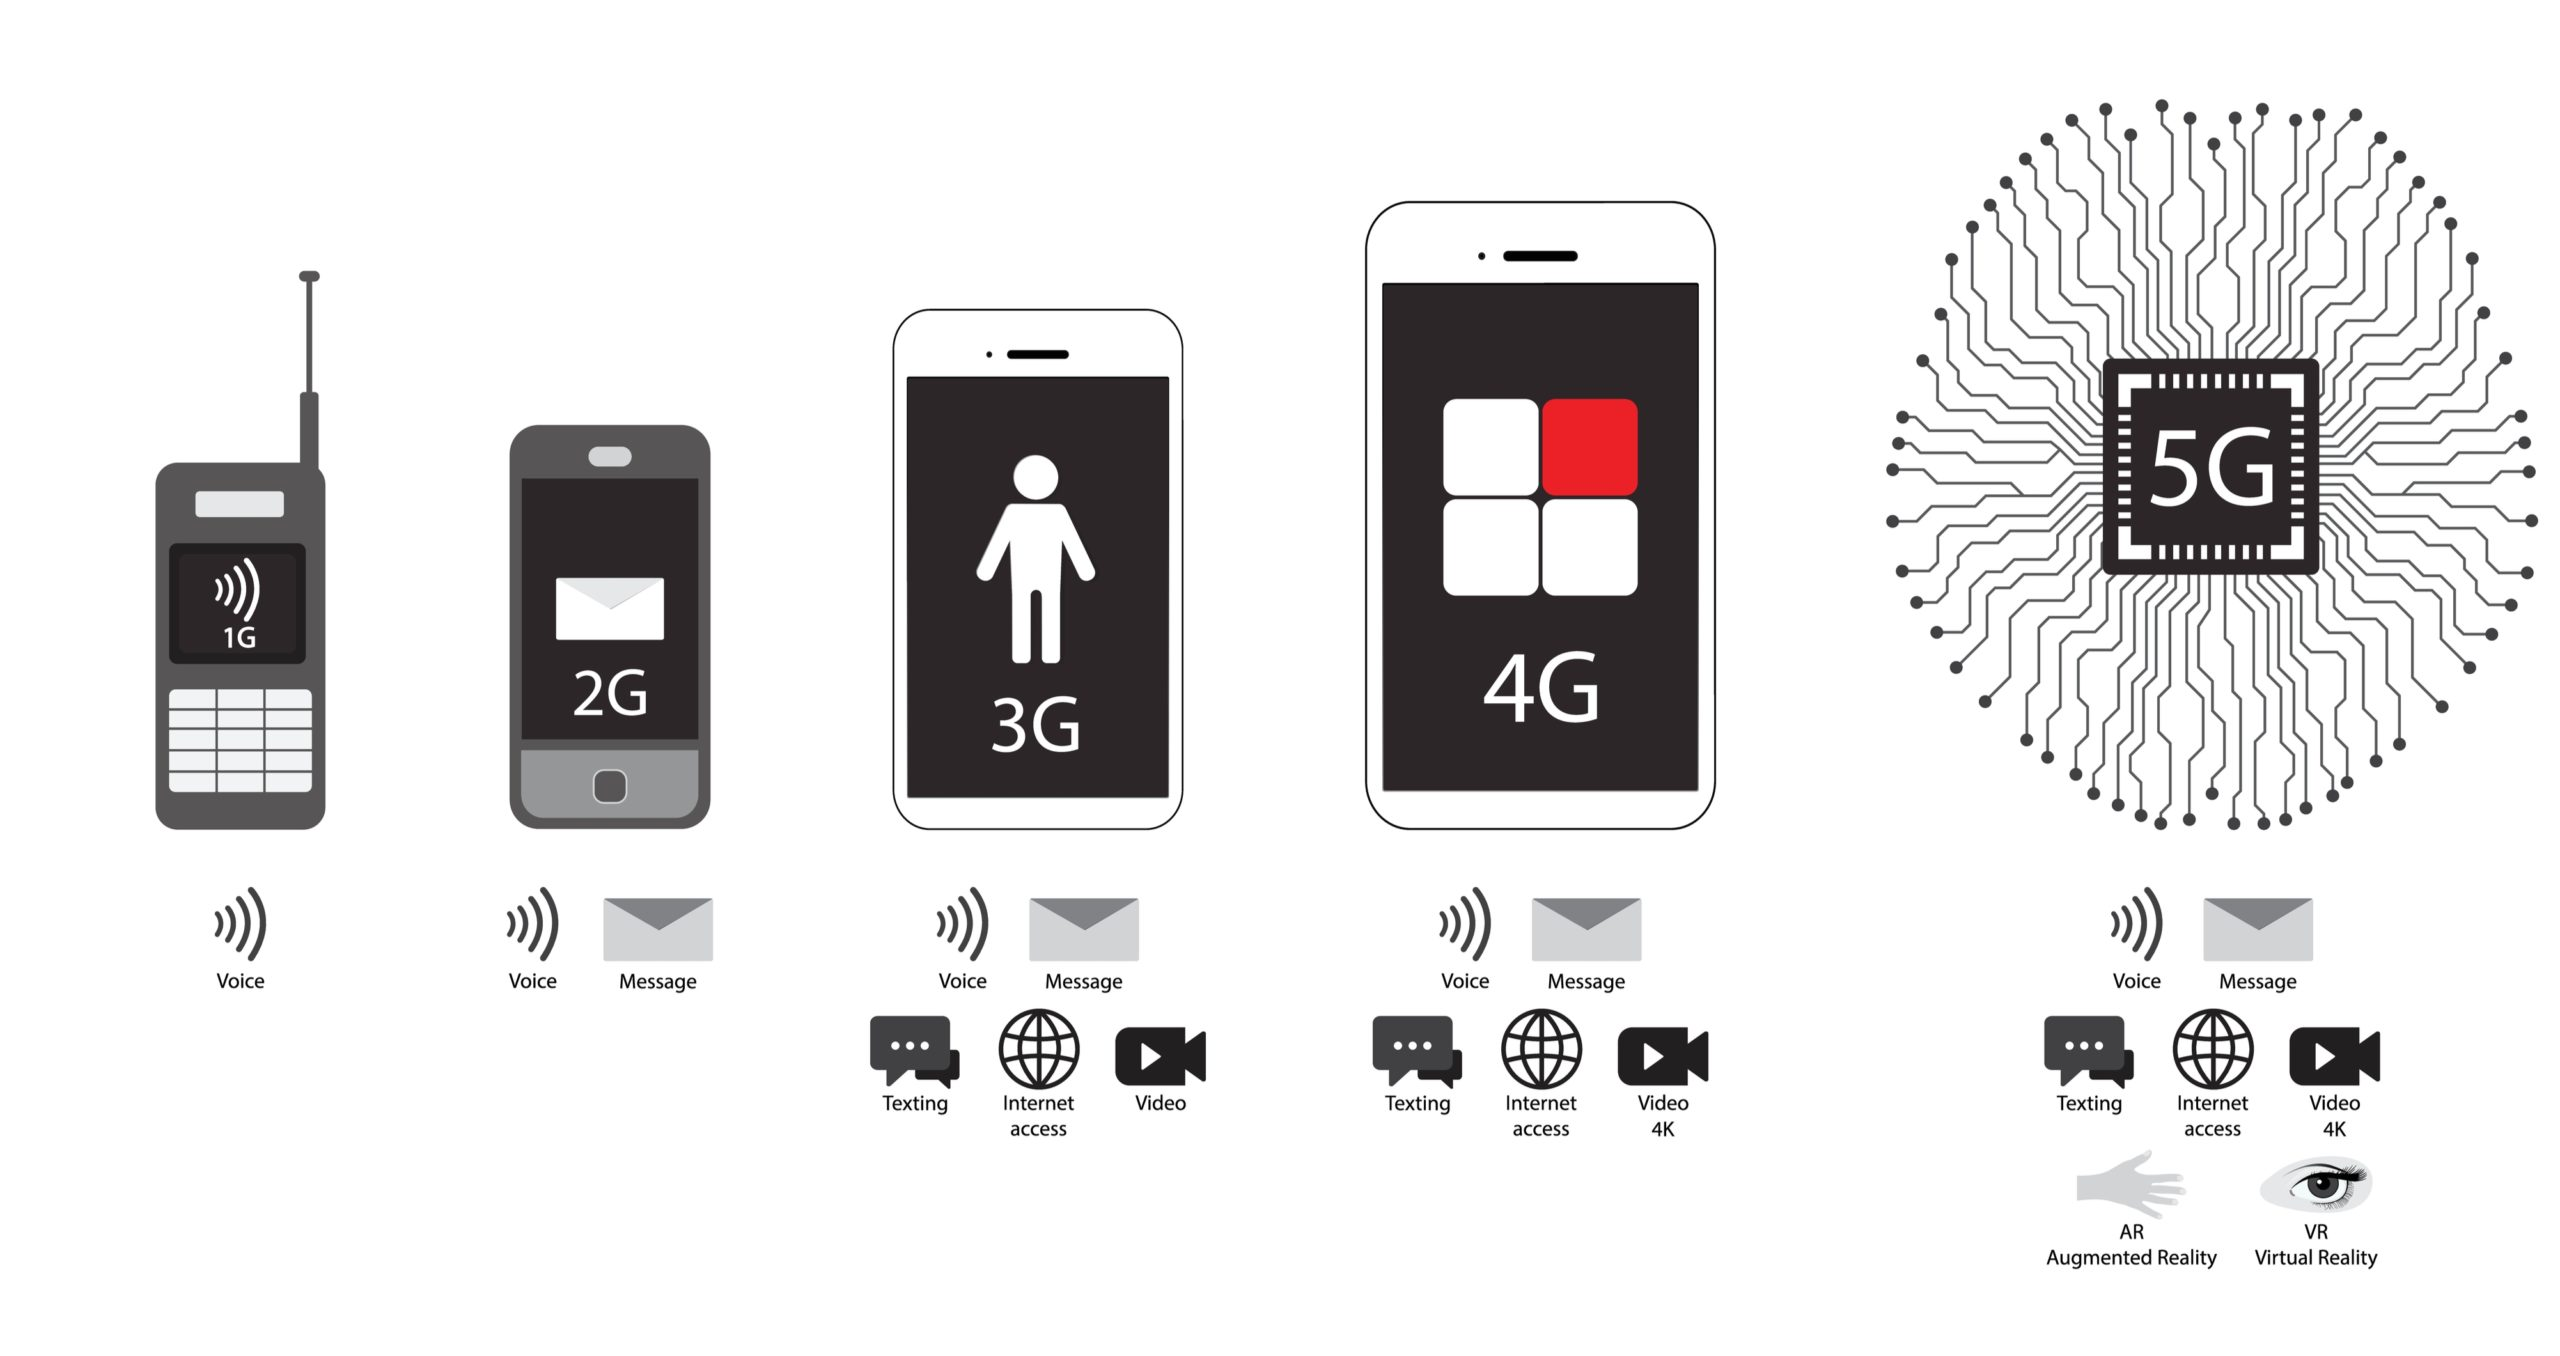
\includegraphics[width=0.7\textwidth]{images/generations-scheme.jpg}
    \caption{Schema delle generazioni cellulari}
\end{figure}

\subsection{1G}
La generazione 1G è uno dei primi standard di comunicazione cellulare. Il suo funzionamento era completamente analogico 
e ormai è stata rimpiazzata totalmente dalle generazioni digitali successive.\\
L'architettura di questa generazione è molto semplice, è composta da tre componenti principali:
\begin{itemize}
    \item Antenne per la trasmissione
    \item \textit{Mobile Telephone Switching Office} (MTSO)
    \item Unità mobile (cellulare)
\end{itemize}
\begin{figure}[ht]
    \centering
    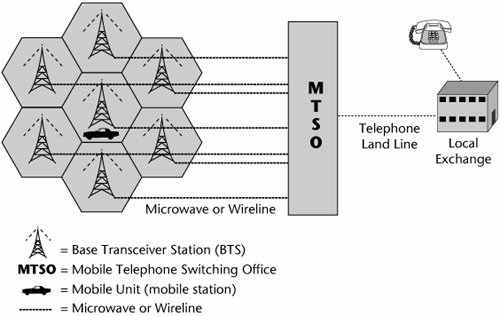
\includegraphics[width=0.7\textwidth]{images/1g.jpg}
    \caption{Architettura 1G}
\end{figure}
Si basava sulla \textit{frequency-division multiple access} (FDMA) in cui ogni dispositivo che si connetteva alla stazione radio
aveva assegnata una specifica sotto banda\cite{generations}.

\clearpage

\subsection{2G}
A differenza della prima generazione, la seconda introuduce per la prima volta una rete completamente digitale.
La seconda generazione cellulare è composta da diverse versioni che si sono susseguite nel corso degli anni aggiungendo nuove 
funzionalità.
Anche la sua architettura subisce delle modifiche, per questo verranno trattate in seguito.
\subsubsection{GSM}
Il GSM, ovvero \textit{Global System for Mobile Communications} è uno standard di seconda generazione che introuduce importanti novità.
Le principali caratteristiche introdotte sono:
\begin{itemize}
    \item Maggiori velocità di trasmissione
    \item Cifratura della comunicazione
    \item Introduzione di nuovi servizi come gli SMS
\end{itemize}
\begin{figure}[ht]
    \centering
    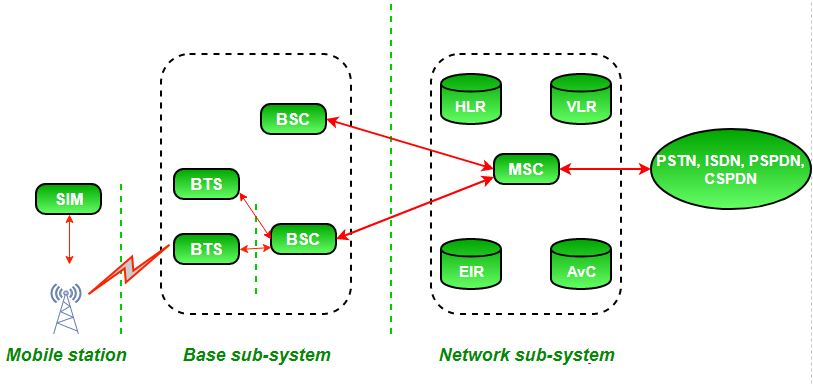
\includegraphics[width=0.7\textwidth]{images/2g-gsm.jpg}
    \caption{Architettura GSM}
\end{figure}
La sua architettura è composta da due macro aree: La BSS \textit{Base Station SubSystem} e la NSS \textit{Network SubSystem}.
Il BSS è l'insieme delle antenne ricevitori, rappresentano il primo collegamento con il MS.\\
Il MS si collega alla BS di riferimento, viene identificato tramite l'HLR \textit{Home Location Register}, ovvero un \textit{database} 
che contiene tutte le informazioni necessarie per la gestione dei \textit{subscribers}. Le chiamate e messaggi vengono smistati nella rete 
telefonica tramite il \textit{Mobile Switching Centre} (MSC).
\subsubsection{GPRS}
La rete \textit{General Packet Radio Service} (GPRS) introduce per la prima volta un trasferimento dati a commutazione di pacchetto per rendere 
possibile l'utilizzo dei servizi \textit{internet} con il proprio dispositivo cellulare\cite{gsm-architecture}.
La sua architettura è la stessa di quella del GSM ma con dei componenti aggiuntivi che consentono la trasmissione dei pacchetti. 
Per esempio, il SGSN \textit{Serving GPRS Support Node} è un componente predisposto per la gestione dei dispositivi connessi alla rete.
\begin{figure}[ht]
    \centering
    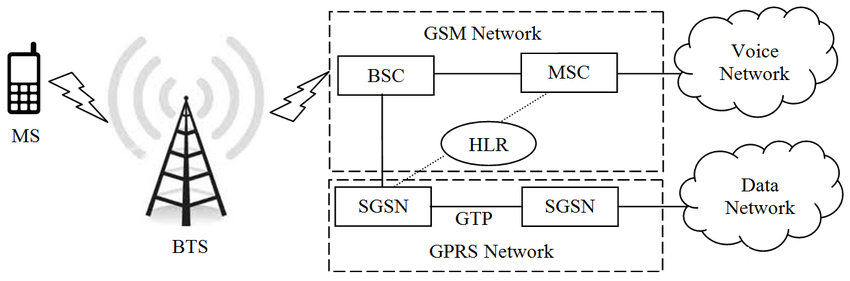
\includegraphics[width=0.7\textwidth]{images/2g-gprs.png}
    \caption{Architettura GPRS}
\end{figure}
\subsubsection{EDGE}
Evoluzione del GPRS che consente maggiori velocità, l'architettura resta invariata.

\clearpage

\subsection{3G}
L'architectura della terza generazione riprende quella già vista nella seconda. Infatti, questa generazione ha avuto come principale obbiettivo 
quello di consolidare l'integrazione della rete internet nei sistemi cellulari ed aumentare le velocità di trasmissione per consentire l'utilizzo 
di nuovi servizi.
Le reti di terza generazione possono essere divise in tre componenti fondamentali:
\begin{itemize}
    \item UE \textit{User equipment}
    \item RNS \textit{Radio Network Subsystem}
    \item \textit{Core Network}
\end{itemize}

\subsubsection{UMTS}
L'UMTS ovvero \textit{Universal Mobile Telecommunications System} è il primo standard di terza generazione.
\begin{figure}[ht]
    \centering
    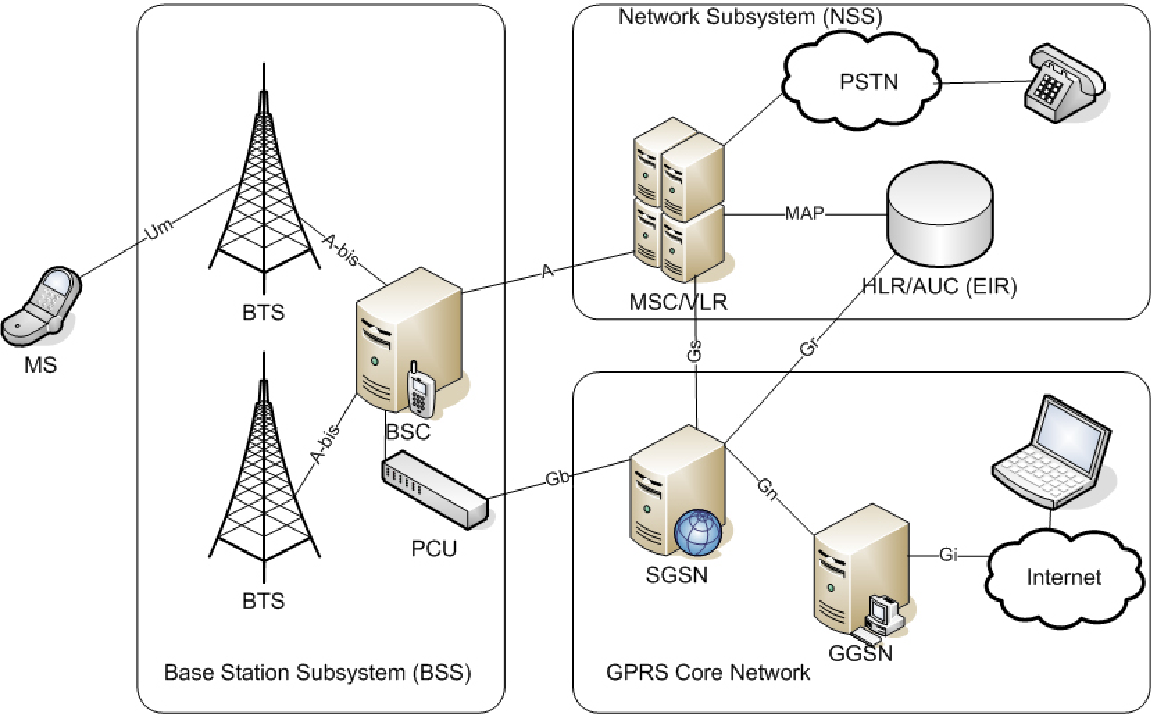
\includegraphics[width=0.7\textwidth]{images/3g-umts.png}
    \caption{Architettura UMTS}
\end{figure}


\subsubsection{HSPA/HSPA+}
Evoluzione del UMTS per consentire velocità maggiori apportando modifiche nella trasmissione del segnale.
Con questo nuovo standard si riescono a raggiungere velocità di 42 Mb/s.

\clearpage

\subsection{4G}

\subsubsection{LTE}
\begin{figure}[ht]
    \centering
    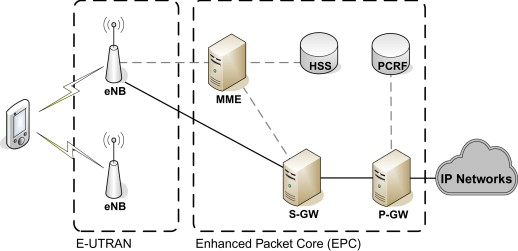
\includegraphics[width=0.8\textwidth]{images/4g-lte.jpg}
    \caption{Architettura LTE}
\end{figure}

\clearpage

\subsection{5G}
Il 5G, ovvero lo standard di quinta generazione rappresenta l'ultima frontiera della tecnologia cellulare.
Il suo principale scopo è consentire l'\textit{Internet of Things} massivo, ossia un \textit{network} che sia 
in grado di gestire la connessione di molti dispositivi con latenze molto piccole.
Per consentire velocità fino a 10 Gb/s si sono
dovute apportare importanti modifiche strutturali che rendono la sua architettura molto diversa da quelle viste fin'ora.\\
L'architettura implementata prende il nome di \textit{Service-Base Architecture} (BSA).
La BSA consiste nel dividere tutte le funzioni in una serie di \textit{microservices}\cite{5g-approach}. 
Questa nuova struttura è stata introdotta per garantire la scalabilità del sistema, migliorare le prestazioni (velocità) e per 
permettere di realizzare il \textit{massive IOT}, che richiede la gestione simultanea di molti dispositivi.\\
I principali blocchi che la compongono sono:
\begin{itemize}
    \item AMF \textit{Core Access and Mobility Management Function} responsabile dell'autenticazione e autenticazione del dispositivo.
    \item SMF \textit{Sesson Management Function} per la gestione della sessione di ogni UE.
    \item PCF\textit{Policy Control Function} per la gestione delle \textit{policy}
    \item UDM \textit{Unified Data Management} per la gestione dell'identità dell'utente, questo compito era precedentemente svolto da HSS o HLR.
    \item AUSF \textit{Authentication Server Function} per effettuare l'autenticazione dell'utente.
    \item SDSF \textit{Structured Data Storage Network Function} è un helper per la memorizzazione di dati strutturati.
    \item UDSF \textit{Unstructured Data Storage Network Function} è un helper per la memorizzazione di dati non strutturati.
    \item NEF \textit{Network Exposure Function} per esporre determinate funzionalità a servizi di terze parti.
    \item NRF \textit{NF Repository Function} per scoprire tutti i servizi disponibili.
    \item NSSF \textit{Network Slicing Selector Function} per selezionare una determinata partizione di \textit{network}.
    \item UPF \textit{User Plane Function} trasporta il traffico dal RAN all'internet.
\end{itemize}
\begin{figure}[ht]
    \centering
    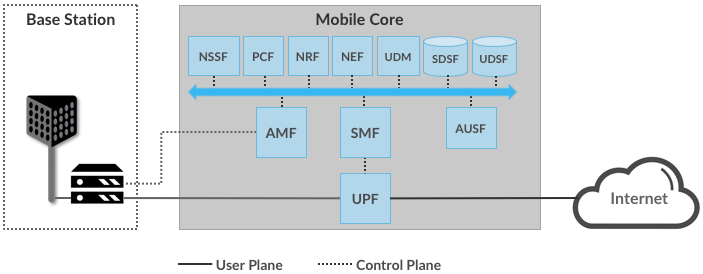
\includegraphics[width=0.8\textwidth]{images/5g-planes.png}
    \caption{Architettura 5G\cite{5g-approach}}
\end{figure}

\clearpage

\subsubsection{Network Slicing}
Il \textit{Network Slicing} rappresenta una delle caratteristiche più importanti del 5G. Con questo termine si intende il partizionamento della
rete in diversi "piani" ciascuno con caratteristiche e requisiti particolari, indipendente e autonomo. Questo risulta fondamentale nella realizzazione 
dell' IOT massivo, infatti in questo modo la gestione del traffico terrà conto dell'applicazione che viene utilizzata nel dispositivo per decidere quali prestazioni sono 
richieste da quel dispositivo.
\begin{figure}[ht]
    \centering
    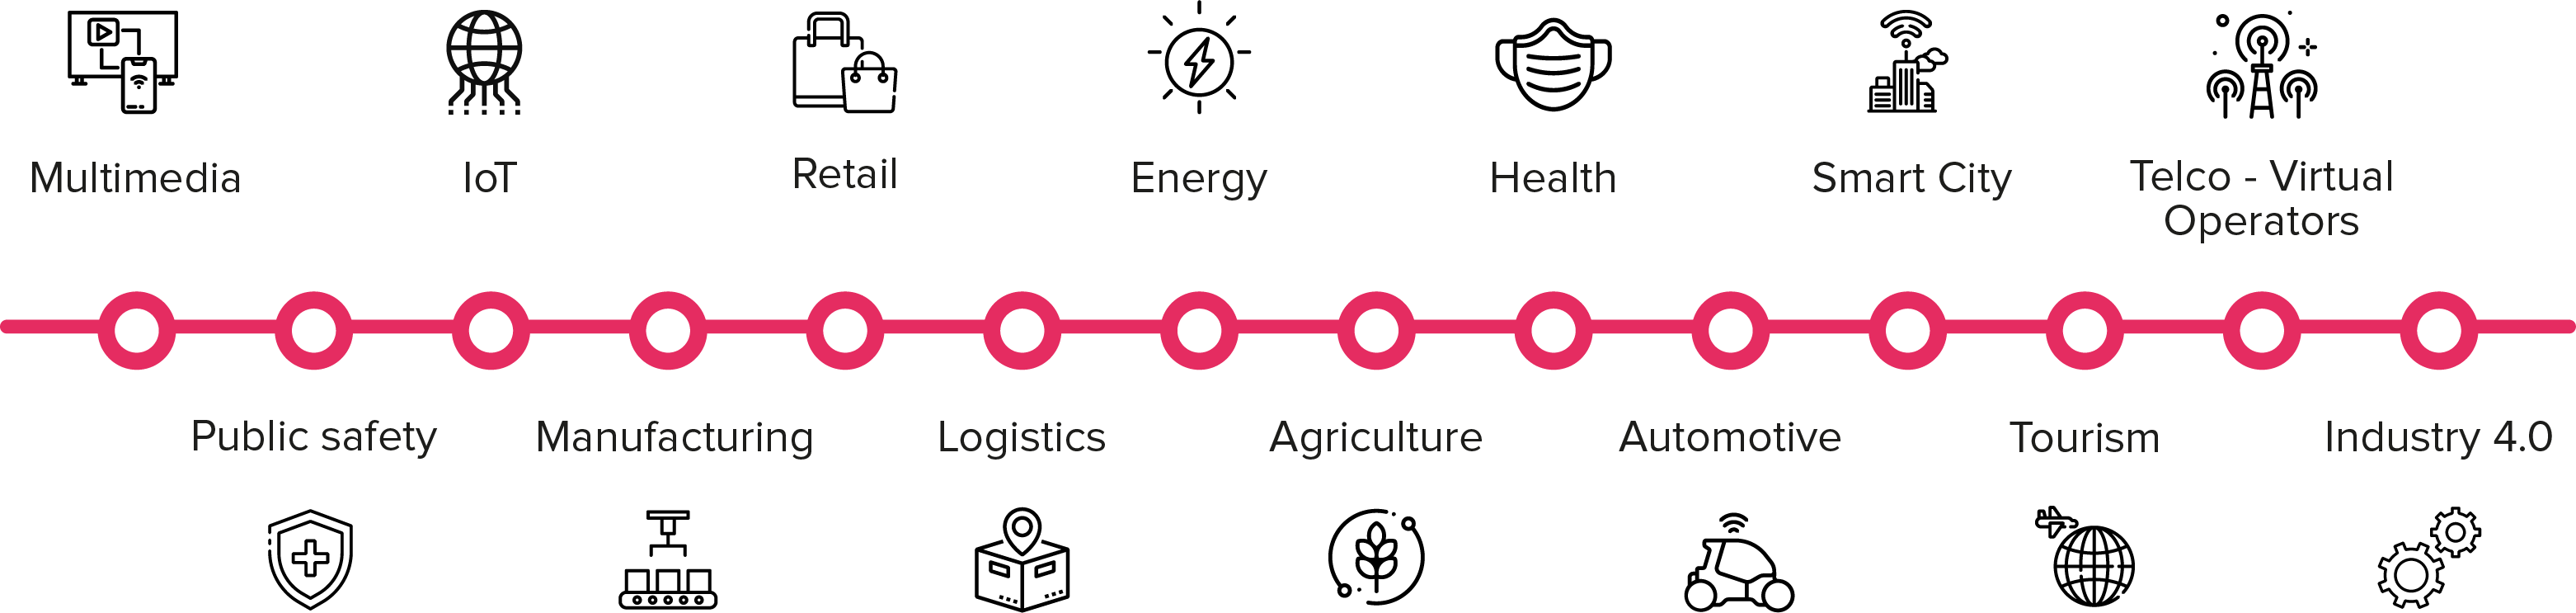
\includegraphics[width=0.8\textwidth]{images/5g-eg-of-use.png}
    \caption{Esempi di applicazioni per il 5G}
\end{figure}\\
La realizzazione del \textit{Network Slicing} avviene tramite i \textit{Software Degined Network} che nella prossima sezione verranno approfonditi.
\subsubsection{Software Defined Network}
I \textit{Software Defined Network} (SDN) sono dei programmi per la virtualizzazione della rete. Sono necessari per interfacciarsi a livello applicativo con i dispositivi cellulari 
in modo da gestire il traffico della rete in modo efficacie\cite{5g-sdn}.
